\subsection*{Binning Methods}
\addcontentsline{toc}{subsection}{Binning Methods}%

The data set $D$ events can be labelled with a typical value interval (the so-called binning size) for every Feature-A value with a slight difference to each other. Binning generation for the events allows us to investigate them in a {\color{red}sequential manufacturing system} and can be performed in alternative ways.

Say that we do the Feature-A values labelling with a typical binning size, in our case, 99, so that all of the events in $D$ must match the corresponding Fixed Step Sized (FSS) interval, as shown in Table~\ref{Tab: D-dataset-FSS}. 
\begin{table}[hb!]
	\centering
	\setlength{\arrayrulewidth}{0.75pt}% 
	\begin{tabular}{|cc|c|ccc|c|}
		\hline \rowcolor[HTML]{FFFFC7}
		\makecell{Event\\ID} 	&& Feature-A    	&& FSS Bins && \makecell{Sequence\\ID}  \\ \hline
		1 	      && 280	    && 200-299	&& 1 		     \\
		2 		  && 250	    && 200-299	&& 1 		     \\
		3 	      && 890	    && 800-899	&& 2 		     \\
		4 		  && 850	    && 800-899	&& 2 		     \\
		\vdots	  && \vdots  	&& \vdots	&& \vdots 	     \\
		n-2 	  && 520	    && 500-599	&& k 		     \\
		n-1       && 630	    && 600-699	&& k 		     \\
		n 		  && 610	    && 600-699	&& k 		     \\ \hline
	\end{tabular}
	\caption{Data Set D with FSS Bin Size Labels.}
	\label{Tab: D-dataset-FSS}
\end{table}

An alternative way of label generation is to create bins with equal event counts per bin among the complete data set; Fixed Bucket Sized (FBS) labelling is shown in Table~\ref{Tab: D-dataset-FBS}.
\begin{table}[ht!]
	\centering
	\setlength{\arrayrulewidth}{0.75pt}% 
	\begin{tabular}{|cc|c|ccc|c|}
		\hline \rowcolor[HTML]{FFFFC7}
		\makecell{Event\\ID} 	&& Feature-A    	&& FBS Bins && \makecell{Sequence\\ID} \\ \hline
		1 	      && 280	    && 200-599	&& 1 		     \\
		2 		  && 250	    && 200-599	&& 1 		     \\
		3 	      && 890	    && 630-899	&& 2 		     \\
		4 		  && 850	    && 630-899	&& 2 		     \\
		\vdots	  && \vdots  	&& \vdots	&& \vdots 	     \\
		n-2 	  && 520	    && 200-599	&& k 		     \\
		n-1       && 630	    && 630-899	&& k 		     \\
		n 		  && 610	    && 600-629	&& k 		     \\ \hline
	\end{tabular}
	\caption{Data Set D with FBS Bin Size Labels.}
	\label{Tab: D-dataset-FBS}
\end{table}
The alternative binning generation methods mentioned above let us derive two distinguished approaches to construct association networks. The first one is the FSS Network approach; it has graph nodes as binning groups with equal bin sizes. Manipulation of binning size allows us to aggregate events in different network nodes. The FBS Network approach is the second one where the network nodes are binning groups with an equal number of events per bin. Defining a typical bucket size for the network nodes results in arbitrary interval boundaries for each node, and it allows to control their population.
 \begin{figure}[!ht]
	\begin{center}
		\makebox[\textwidth]{
			\centering
			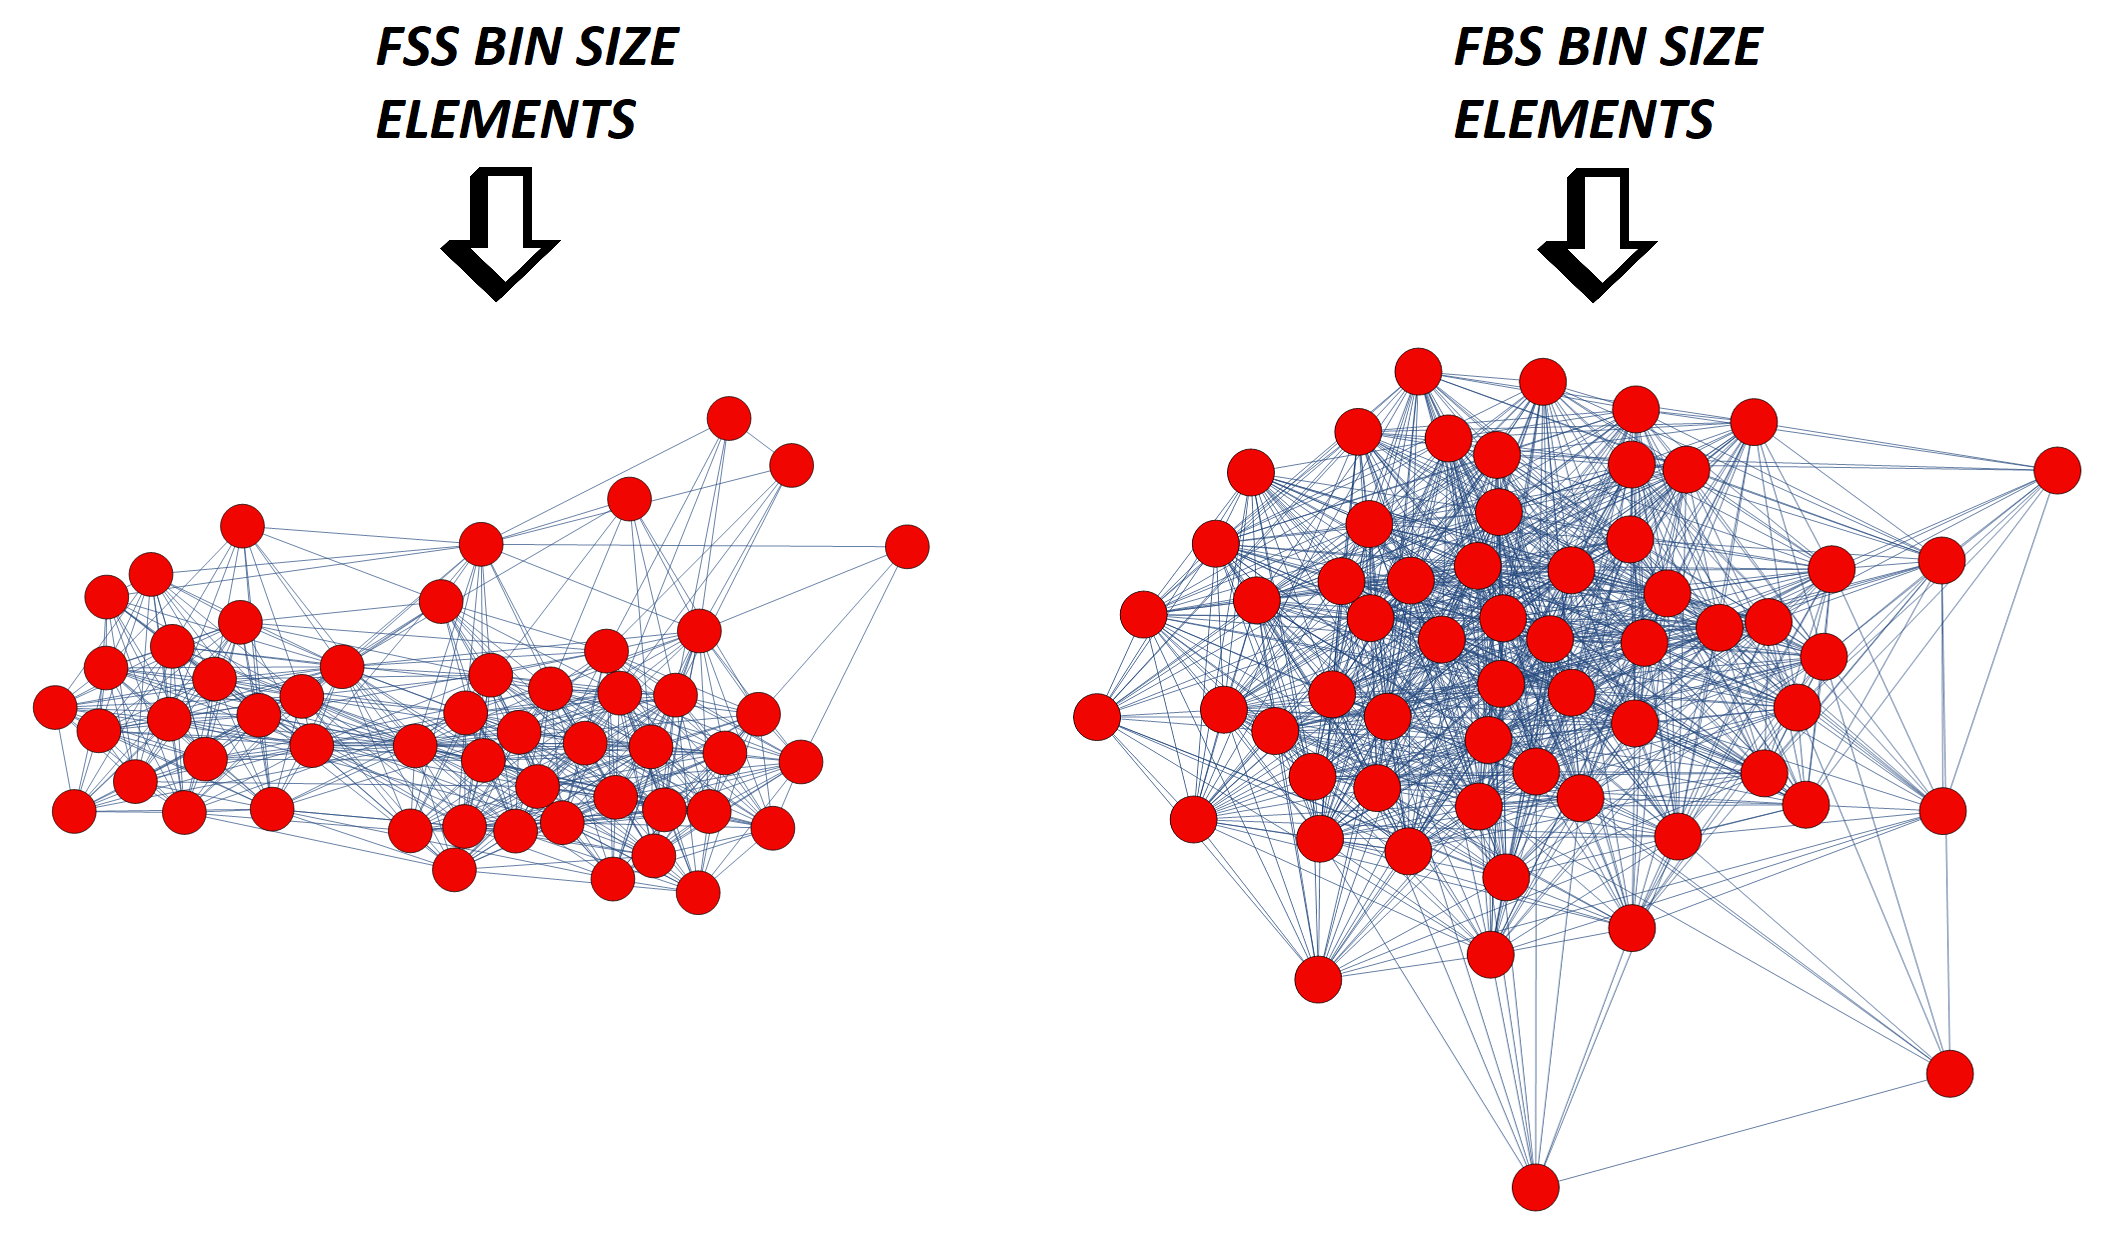
\includegraphics[width=0.8\linewidth]{../images/methodology-association-networks-hyp_networks.png}}
		\caption{Graph Results For Two Different Network Approaches.}
		\label{figure-hyp_graphs}
	\end{center}
\end{figure}

{\color{red}FSS and FBS networks generation for the production events underlie the developed hypothesis of this thesis work: Non-random features of the association networks derived from these two methods.}